\documentclass[12pt,a4paper]{article}

\usepackage[utf8]{inputenc}
\usepackage{graphicx}
\usepackage{float}

\begin{document}

\title{MI-PAA 2015 4.ukol \\
}
\author{Tomas Nesrovnal\\nesrotom@fit.cvut.cz}
\date{\today}
\maketitle

\section{Zvolený algoritmus}
Simulovaná evoluce

\subsection{Jedinec}
Jedinec v populaci je jednorozmerne bitove pole, kdy jednotlivy bit znaci pritomnost predmetu v batohu.

\subsection{Fitness}
Zde jsem zvolil jednoduche a primocare reseni a to, ze fitness jedince je celkova cena. Pokud je prekrocena kapacita, je fitness 0.

Mozne vylepseni by bylo priradit kladnou fitness i nevalidnim resenim, ale s dobrym potencialem.

\subsection{Inicializace}
Kazdy jedinec je nahodne generovan (kazdy bit ma 50 \% sanci byt 1) do te doby, dokud nebude mit $fitness > 0$.

\subsection{Crossover}
Jednobodove a dvoubodove krizeni.

\subsection{Mutace}
Pri mutaci je s jistou (velmi malou) pravdepodobnosti zmutovan kazdy jedinec.

\subsection{Selekce}
Turnajova selekce.

\subsection{Vliv nahody}
Pred kazdym merenim byla vyresetovana nahoda. Protoze je implementace v C, vola se srand(0).


\section{Na cem bylo mereno}
Intel(R) Core(TM) i3-2328M Processor (3M Cache, 2.20 GHz), gcc 4.9.2 (-Ofast), OS GNU/Linux Lubuntu 14.04 64bit




\section{Citlivost FPTAS na cenu}
Protoze implementace dynamickeho programovani pouzivala dekompozici podle vahy, k mereni byl pouzit FPTAS s $eps=0$, ktery pouziva dekompozici podle ceny.
\begin{figure}[H]
	\caption{Citlivost na cenu. Cas FPTASu s nulovou chybou.}
 	\centerline{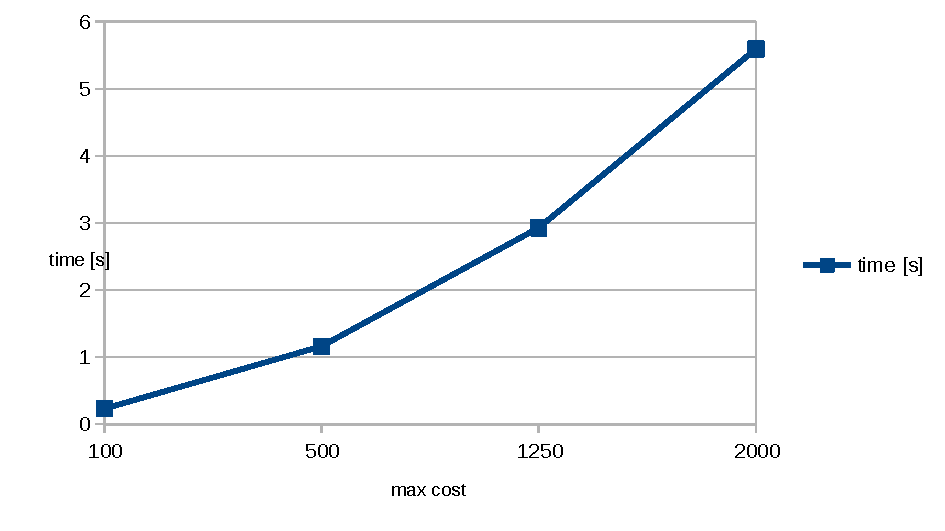
\includegraphics{./fptas_cost.pdf}}
\end{figure}

\section{Citlivost dynamickeho programovani na vahu}

\begin{figure}[H]
	\caption{Citlivost na vahu. Dynamicke programovani s dekompozici podle vahy.}
 	\centerline{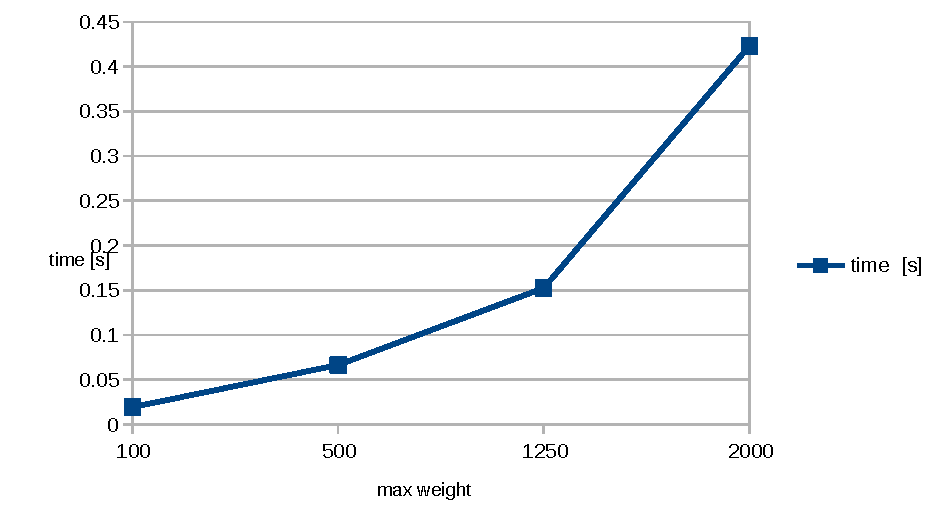
\includegraphics{./h_weight.pdf}}
\end{figure}

\section{Vliv pomeru kapacity k sumarni vaze na heuristiku}

Se zvysujicim se paremetrem m klesala relativni chyba  jak u heuristiky podle pomeru ceny a vahy tak i heuristiky jen podle ceny.

\section{Zaver}
Zjednodusene by se dalo rict, ze experimenty potvrdily to, ze zadna z metod neni obecne lepsi nez ostatni. Zavislost na druhu dat dokaze zmenit mnoho faktoru.

%%%%%%%%%%%%%%%%%%%%%%%%%%%%%%%%%%%%%%%%%%%%%%%%%%%%%%%%%%%%%%%%%%%%%%%%%%%%%%
\end{document}
